\setcounter{Exercise}{0}

\section*{Algorithme et arbres binaires de recherches}
On peut implémenter un arbre binaire en Python comme un tableau, pour ce faire chaque nœud est représenté par une liste contenant sa valeur, son sous-arbre gauche et son sous-arbre droit.
Par exemple :
\begin{lstlisting}{style=pythonstyle, language=Python}
arbre = [20, 
            [7, 
                [4,
                    [2, None, None],
                    None],
                [15,
                    [5, None, None],
                    None]],
            [53,
                [46,
                    [29, None, None],
                    None],
                [80,
                    [74, None, None],
                    None]]]            
\end{lstlisting}
Donne l'arbre :
\begin{center}
    \begin{center}
    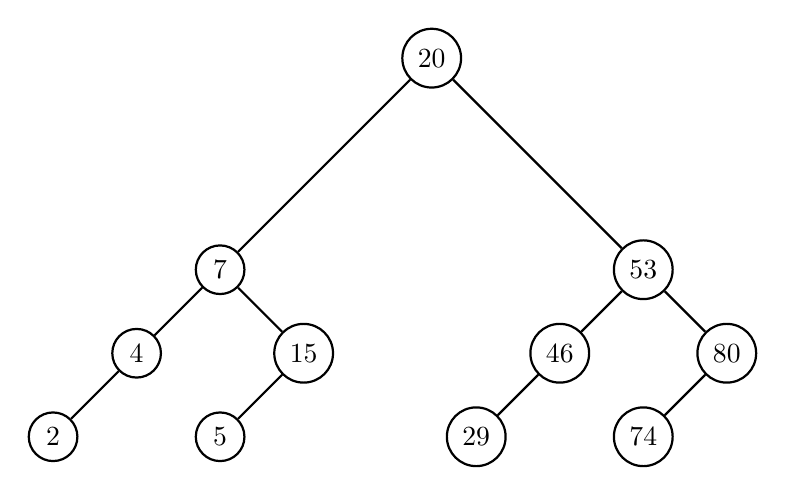
\begin{tikzpicture}[node distance={1.5cm}, thick, main/.style = {draw, circle}] 
    \node[main] (20) {20}; 
    \node[main] (7) [below left of = 20, node distance={3.8cm}] {7}; 
    \node[main] (53) [below right of = 20, node distance={3.8cm}] {53}; 
    \node[main] (4) [below left of = 7] {4}; 
    \node[main] (15) [below right of = 7] {15}; 
    \node[main] (2) [below left of = 4] {2}; 
    \node[main] (5) [below left of =  15] {5}; 
    \node[main] (46) [below left of = 53] {46}; 
    \node[main] (80) [below  right of = 53] {80}; 
    \node[main] (29) [below left of = 46] {29}; 
    \node[main] (74) [below right of=  46] {74}; 
    \draw (20) -- (7); 
    \draw (20) -- (53); 
    \draw (7) -- (4); 
    \draw (7) -- (15); 
    \draw (4) -- (2); 
    \draw (15) -- (5);
    \draw (53) -- (46);
    \draw (53) -- (80);
    \draw (46) -- (29);
    \draw (80) -- (74);
    \end{tikzpicture} 
\end{center}


\end{center}
Pour la suite des exercices, nous considérerons toujours cette implémentation de la classe arbre.

\begin{Exercise}[title={Dessinons}]

\Question Dessiner l'arbre correspondant au code ci-dessous.\\
\emptybox{5cm}
\begin{lstlisting}{style=pythonstyle, language=Python}
arbre = [8, [3, [1, None, None], [6, [4, None, None], [7, None, None]]], [10, None, [14, [13, None, None], None]]]
\end{lstlisting}

\Question Est-ce un arbre binaire de recherche ?

\Question Compléter le code ci-dessous permettant de créer l'arbre avec une variable par nœud  ?\\
\begin{lstlisting}{style=pythonstyle, language=Python}
n13 = [13, None, None]
n1 = [1, None, None]
n4 = ....
n7 = ....
n6 = [6, n4, n7]
....
....
....
....
\end{lstlisting}

\Question Appliquez le parcours infixe à cet arbre, que remarquez-vous  ?\\
\emptybox{1cm}
\end{Exercise}

\begin{Exercise}[title={A la recherche du logarithme}]

\Question Compléter le code ci-dessous permettant d'insérer un élément dans un arbre binaire de recherche ?\\
\begin{lstlisting}{style=pythonstyle, language=Python}
def insertionABRnr(arbre,element):
    arbre_suivant = arbre
    while arbre_suivant is not None:
        arbre = ............
        if .....................:
            arbre_suivant = arbre[1]
        if .....................:
            arbre_suivant = arbre[2]
    if arbre[0] > element:
        arbre[1] = ...............
        print(element, 'ajouté à gauche de', arbre[0])
    if arbre[0] < element:
        arbre[2] = ...............
        print(element, 'ajouté à droite de', arbre[0])
\end{lstlisting}

\Question Cet algorithme est-il récursif ?\\

\Question On souhaite implémenter cette fonction permettant de rechercher un élément dans un arbre binaire de recherche de manière récursive, compléter le code suivant ?\\
\begin{lstlisting}{style=pythonstyle, language=Python}
def rechercheABR(arbre,element):
    if arbre is None:
        .............
    else:
        if arbre[0] == element:
            return True
        if ........................:
            return ........................
        if ........................:
            return ........................
\end{lstlisting}
\end{Exercise}
\pagebreak